\documentclass[10pt]{article}
\usepackage[margin=0.65in]{geometry}
\usepackage[T1]{fontenc}
\usepackage{lmodern}
\usepackage{amsmath,amssymb}
\usepackage[table]{xcolor}
\usepackage{array,tabularx,longtable,multirow,booktabs}
\usepackage{tikz}
\usetikzlibrary{arrows.meta,positioning,shapes.geometric,calc}
\usepackage[most]{tcolorbox}
\usepackage{enumitem}
\usepackage{ragged2e}
\usepackage{graphicx}
\usepackage{microtype}
\usepackage{titlesec}
\usepackage{hyperref}

\definecolor{navy}{HTML}{202F73}
\definecolor{blue}{HTML}{155B9C}
\definecolor{midblue}{HTML}{427ED7}
\definecolor{paleblue}{HTML}{C9D9F2}
\definecolor{teal}{HTML}{165A64}
\definecolor{burgundy}{HTML}{7A1945}
\definecolor{brick}{HTML}{98240F}
\definecolor{orange}{HTML}{BF6900}
\definecolor{gold}{HTML}{8D7000}
\definecolor{green}{HTML}{347B22}
\definecolor{palegreen}{HTML}{B7D7A8}
\definecolor{lightgreen}{HTML}{D9EAD3}
\definecolor{paleyellow}{HTML}{FFF2CC}
\definecolor{paleorange}{HTML}{FCE5CD}
\definecolor{palered}{HTML}{F4CCCC}
\definecolor{lightgray}{HTML}{F0F1F4}
\definecolor{medgray}{HTML}{A6A6A6}
\definecolor{cyanlearn}{HTML}{64D8DE}
\definecolor{greenlearn}{HTML}{B7E39D}
\definecolor{yellowlearn}{HTML}{FFE89A}

\hypersetup{colorlinks=true,linkcolor=navy,urlcolor=blue}
\setlength{\parindent}{0pt}
\setlength{\parskip}{0.55\baselineskip}
\setlist[itemize]{leftmargin=1.4em,itemsep=1pt,topsep=2pt}
\setlist[enumerate]{leftmargin=1.6em,itemsep=1pt,topsep=2pt}
\renewcommand{\arraystretch}{1.16}
\titleformat{\section}{\LARGE\bfseries\color{navy}}{}{0pt}{}
\titleformat{\subsection}{\Large\bfseries}{}{0pt}{}
\titleformat{\subsubsection}{\large\bfseries\color{navy}}{}{0pt}{}

\newcolumntype{L}[1]{>{\RaggedRight\arraybackslash}p{#1}}
\newcolumntype{Y}{>{\RaggedRight\arraybackslash}X}
\newcommand{\sourceheading}[2]{%
  {\Huge\bfseries\itshape\color{navy} #1}\par
  {\huge\bfseries #2}\par}
\newcommand{\visualexplanation}[1]{%
  \begin{tcolorbox}[colback=lightgray,colframe=navy!35,boxrule=0.5pt,
    arc=2mm,left=2mm,right=2mm,top=1.5mm,bottom=1.5mm]
  \textbf{Visual explanation.} #1
  \end{tcolorbox}}
\newcommand{\smallhead}[1]{\textbf{\color{navy}#1}}
\newcommand{\weekhead}[1]{\cellcolor{navy}\color{white}\bfseries #1}
\newcommand{\coursehead}[1]{\rowcolor{navy}\color{white}\bfseries #1}

\begin{document}

\begin{center}
\vspace*{2.2cm}
{\fontsize{42}{48}\selectfont\bfseries\color{white}\colorbox{navy}{\strut 02}}\\[1.2cm]
{\fontsize{34}{40}\selectfont\bfseries\color{navy}Learning Journey \& Courses Plan}
\end{center}

\vspace{1.2cm}
\begin{tcolorbox}[colback=navy,colframe=navy,arc=3mm]
\centering\color{white}\Large
Prepared by SBM ITB --- Direktorat Pendidikan Profesional Berkelanjutan
\end{tcolorbox}

\section{Learning Journey: 5-Components for Transformation}

\emph{Ekosistem 5-komponen terintegrasi untuk mengubah potensi pelajar menjadi \textbf{strategic business leader} dengan kemampuan memimpin dan eksekusi}

\begin{tcolorbox}[colback=paleblue,colframe=navy,title=Integrated Design Logic,
  fonttitle=\Large\bfseries,arc=2mm]
Program ini tidak hanya terdiri dari kelas \emph{stand-alone}, namun mengintegrasikan kurikulum, metode pembelajaran, projek bisnis real, mentoring, teknologi, dan lingkungan kampus residensial dalam satu arsitektur pengembangan.
\end{tcolorbox}

\begin{tcolorbox}[colback=palered!55,colframe=brick,
  title={\Large 1 \quad Desain Kurikulum\quad\small\itshape 3 Learning Building Blocks},fonttitle=\bfseries]
\begin{tabularx}{\linewidth}{Y Y Y}
\textbf{1 --- Foundation Learning}\newline
Learning agility $\bullet$ Communication $\bullet$ Professional presence $\bullet$ Strategic thinking $\bullet$ Basic accounting $\bullet$ Management fundamentals
&
\textbf{2 --- 6 Core Courses}\newline
6 MK inti: OB \& MP, Financial Management \& Strategy, Marketing Management, OSCM, Strategic Decision Making \& Negotiation dalam 6 sektor BUMN
&
\textbf{3 --- Managerial, Leadership, Entrepreneurship}\newline
Managerial skill $\bullet$ Leadership skill $\bullet$ Entrepreneurship as capability to lead, manage, and create value
\end{tabularx}
\end{tcolorbox}

\begin{center}\color{navy}\Large$\downarrow$\end{center}

\begin{tcolorbox}[colback=palered!35,colframe=red!70!black,
  title={\Large 2 \quad Metode Pembelajaran\quad\small\itshape Case-based \& blended exposure},fonttitle=\bfseries]
\begin{tabularx}{\linewidth}{Y Y Y}
\textbf{Core Method}\newline
Pembelajaran Case-based $\bullet$ Studi kasus $\bullet$ Diskusi $\bullet$ Simulasi $\bullet$ Gamifikasi $\bullet$ Refleksi
&
\textbf{Learning Reinforcement}\newline
Pra-pembelajaran via LMS $\bullet$ Rencana studi dan rekap mingguan $\bullet$ Leader talks $\bullet$ Business sharing $\bullet$ Company visit
&
\textbf{Perspektif}\newline
Kombinasi academic rigor + business relevance + national context + global perspective
\end{tabularx}
\end{tcolorbox}

\begin{center}\color{navy}\Large$\downarrow$\end{center}

\begin{tcolorbox}[colback=paleorange,colframe=orange,
  title={\Large 3 \quad Action Learning Project\quad\small\itshape Isu bisnis nyata BUMN},fonttitle=\bfseries]
\begin{center}
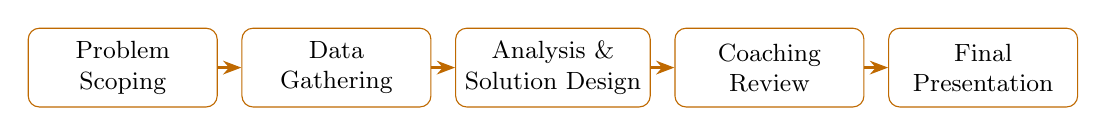
\begin{tikzpicture}[node distance=3mm, every node/.style={font=\small,align=center}]
\node[draw=orange,fill=white,rounded corners,minimum width=2.4cm,minimum height=1cm] (a) {Problem\\Scoping};
\node[draw=orange,fill=white,rounded corners,right=of a,minimum width=2.4cm,minimum height=1cm] (b) {Data\\Gathering};
\node[draw=orange,fill=white,rounded corners,right=of b,minimum width=2.4cm,minimum height=1cm] (c) {Analysis \&\\Solution Design};
\node[draw=orange,fill=white,rounded corners,right=of c,minimum width=2.4cm,minimum height=1cm] (d) {Coaching\\Review};
\node[draw=orange,fill=white,rounded corners,right=of d,minimum width=2.4cm,minimum height=1cm] (e) {Final\\Presentation};
\foreach \x/\y in {a/b,b/c,c/d,d/e}{\draw[-{Stealth},thick,orange] (\x)--(\y);}
\end{tikzpicture}
\end{center}
\textbf{SMART Gate \& Impact}\quad
\textcircled{S}pecific \textcircled{M}easurable \textcircled{A}chievable \textcircled{R}elevant \textcircled{T}ime-Bound.\\
\emph{Output:} Rekomendasi implementasi, estimasi \emph{business impact}, dan rencana \emph{follow-up}.
\end{tcolorbox}

\begin{center}\color{navy}\Large$\downarrow$\end{center}

\begin{tcolorbox}[colback=paleyellow,colframe=gold,
  title={\Large 4 \quad Sistem Mentoring\quad\small\itshape Arsitektur pendukung berlapis},fonttitle=\bfseries]
\begin{tabularx}{\linewidth}{Y Y Y Y Y}
\textbf{SBM ITB}\newline Kedalaman akademik \& praktisi &
\textbf{Mentor Bisnis BUMN}\newline Konteks industri \& realitas eksekusi &
\textbf{Business Coach}\newline Kualitas proses berpikir \& perkembangan kepemimpinan &
\textbf{Pengasuh}\newline Menjaga disiplin, karakter, \& konsistensi berperilaku &
\textbf{Project Owner}\newline Memastikan isu yang dikerjakan relevan bagi BUMN
\end{tabularx}
\end{tcolorbox}

\begin{center}\color{navy}\Large$\downarrow$\end{center}

\begin{tcolorbox}[colback=lightgreen,colframe=green,
  title={\Large 5 \quad Operasional \& Fasilitas\quad\small\itshape Infrastruktur pembelajaran terpercaya},fonttitle=\bfseries]
\begin{tabularx}{\linewidth}{Y Y}
\textbf{Operasional Program}\newline
Jadwal $\bullet$ Alokasi kelas $\bullet$ Fakultas \& fasilitator $\bullet$ Mentoring/coach system $\bullet$ LMS/tools $\bullet$ Evaluasi $\bullet$ Koordinasi logistik
&
\textbf{Nawasena Living-Learning Environment}\newline
Jadwal $\bullet$ Auditorium $\bullet$ Perpustakaan $\bullet$ Klinik 24 jam $\bullet$ Ahli nutrisi $\bullet$ Konseling $\bullet$ Workshop $\bullet$ Akomodasi $\bullet$ Makan $\bullet$ Olahraga $\bullet$ Laundry $\bullet$ Asistensi partisipasi
\end{tabularx}
\end{tcolorbox}

\begin{tcolorbox}[colback=paleblue,colframe=navy,title=Target Outcome,fonttitle=\Large\bfseries]
\textbf{Partisipan yang dapat memahami persoalan, mengambil keputusan yang bertanggung jawab, bekerja lintas fungsi, dan menghasilkan solusi yang berdampak.}
\hfill\colorbox{navy}{\color{white}\bfseries\strut LEARN $\boldsymbol\cdot$ LEAD $\boldsymbol\cdot$ EXECUTE.}
\end{tcolorbox}

\visualexplanation{The diagram is a top-to-bottom integrated design. Curriculum supplies the content; learning methods determine how that content is experienced; the Action Learning Project applies it to a real BUMN issue; the layered mentoring system supports judgment and execution; and operations and facilities make the entire experience possible. All five components converge on the target outcome: a participant who understands problems, makes responsible decisions, works across functions, and produces solutions with measurable impact.}

\section{Learning Journey: 70--20--10 Learning Model}

\begin{tabularx}{\textwidth}{Y Y}
\begin{tcolorbox}[colback=white,colframe=red!45,title=Weekly Study Plan/Recap,fonttitle=\bfseries]
Peserta melakukan asesmen dan evaluasi terhadap materi pembelajaran pada minggu sebelumnya, dan melakukan rencana studi pada minggu tersebut.

\emph{Dilakukan di Kampus DCU Nawasena, didampingi oleh asisten kelas}
\end{tcolorbox}
&
\begin{tcolorbox}[colback=white,colframe=red!35,title=Pre-Learning,fonttitle=\bfseries]
Peserta melakukan persiapan mandiri dengan mempelajari materi, studi kasus, maupun diskusi bersama grup untuk topik yang akan dibawakan pada minggu tersebut.

\emph{Dilakukan di Kampus DCU Nawasena, didampingi oleh asisten kelas}
\end{tcolorbox}
\\
\begin{tcolorbox}[colback=white,colframe=orange!45,title=Lecturing,fonttitle=\bfseries]
Tim pengajar (Dosen) dari SBM ITB membawakan materi dengan skema pembelajaran luring di setiap kelas terkait dengan topik sesuai dengan jadwal kurikulum.

\emph{Pengajaran secara luring oleh Dosen SBM ITB, didampingi oleh asisten kelas, didukung oleh asisten mata kuliah}
\end{tcolorbox}
&
\begin{tcolorbox}[colback=white,colframe=yellow!70!orange,title=Case Study \& Roleplay,fonttitle=\bfseries]
Peserta akan diberikan \emph{case study paper} untuk dipelajari, didiskusikan bersama grup, dan dikerjakan untuk dilakukan pembahasan dan evaluasi kasus.

\emph{Didampingi oleh asisten kelas, modul menggunakan case study Harvard Business School}
\end{tcolorbox}
\\
\begin{tcolorbox}[colback=white,colframe=green!55,title=Group Discussion ALP,fonttitle=\bfseries]
Peserta melakukan diskusi di dalam grup untuk mempersiapkan kegiatan ALP terhadap kasus nyata dengan menerapkan teori yang sudah didapatkan.

\emph{Rangkaian ALP akan didampingi oleh asisten kelas, project owner, dan coach/mentor}
\end{tcolorbox}
&
\begin{tcolorbox}[colback=white,colframe=teal!45,title=Group Discussion Social Project,fonttitle=\bfseries]
Peserta melakukan diskusi di dalam grup untuk mempersiapkan proyek sosial yang akan dilaksanakan pada bulan ke-4 untuk menerapkan teori yang sudah didapatkan.

\emph{Rangkaian SP akan didampingi oleh asisten kelas, pengasuh, dan coach/mentor}
\end{tcolorbox}
\\
\begin{tcolorbox}[colback=white,colframe=midblue!55,title=Kegiatan Khusus,fonttitle=\bfseries]
Peserta mengikuti pembelajaran pelengkap dengan berbagai metode, seperti \emph{Executive Seminar}, \emph{Guest Lecture} CEO BUMN, \emph{Panel Discussion}, maupun \emph{Reflection Session}.

\emph{Kegiatan khusus dapat dilakukan dalam auditorium bersama seluruh peserta, didampingi oleh asisten kelas}
\end{tcolorbox}
&
\begin{tcolorbox}[colback=white,colframe=blue!45,title=Business Immersion,fonttitle=\bfseries]
Peserta akan turun langsung keluar kelas untuk belajar secara imersif dengan sistem praktik/magang dan \emph{company visit} BUMN.

\emph{Kegiatan dilakukan di luar Kampus DCU Nawasena, akan dilakukan asesmen dengan laporan dan presentasi akhir}
\end{tcolorbox}
\end{tabularx}

\visualexplanation{The eight cards describe the recurring learning settings. The first four organize preparation, classroom instruction, and case application; the two group-discussion formats connect theory to the Action Learning Project and Social Project; special activities add executive exposure and reflection; and Business Immersion moves learning into BUMN practice. The italic line in each card identifies the location or the people who accompany that activity.}

\begin{center}
\small
\begin{tabularx}{\textwidth}{Y c c c L{3.1cm}}
\rowcolor{navy}\color{white}\bfseries Kegiatan & \color{white}\bfseries Jumlah Sesi/Minggu & \color{white}\bfseries Total Minggu & \color{white}\bfseries Total Sesi Selama Program & \color{white}\bfseries Kategori Metode Pembelajaran\\
Weekly Study Plan/Recap & 2 & 14 & 28 & \cellcolor{yellowlearn}Experiential Learning\\
\multirow{2}{*}{Pre-Learning} & 2 & 14 & 28 & \cellcolor{cyanlearn}Formal Learning\\
 & 10 & 14 & 140 & \cellcolor{greenlearn}Social Learning\\
Lecturing & 6 & 14 & 84 & \cellcolor{cyanlearn}Formal Learning\\
\multirow{2}{*}{Case Study} & 2 & 14 & 28 & \cellcolor{greenlearn}Social Learning\\
 & 10 & 14 & 140 & \cellcolor{yellowlearn}Experiential Learning\\
Group Discussion ALP & 4 & 14 & 56 & \cellcolor{yellowlearn}Experiential Learning\\
Group Discussion Social Project & 4 & 14 & 56 & \cellcolor{yellowlearn}Experiential Learning\\
\multirow{2}{*}{Kegiatan Khusus} & 2 & 14 & 28 & \cellcolor{greenlearn}Social Learning\\
 & 6 & 14 & 48 & \cellcolor{yellowlearn}Experiential Learning\\
Business Immersion & 40 & 9 & 360 & \cellcolor{yellowlearn}Experiential Learning\\
\end{tabularx}
\end{center}

\visualexplanation{The activity table preserves the source's merged entries for Pre-Learning, Case Study, and Kegiatan Khusus because each of those activities contributes to two learning categories. The weekly frequency and program duration produce the displayed total sessions. Color identifies the method category: cyan for formal learning, green for social learning, and yellow for experiential learning. Business Immersion is the most intensive single activity at 40 sessions per week over nine weeks, while several 14-week activities maintain continuity throughout the program.}

\begin{center}
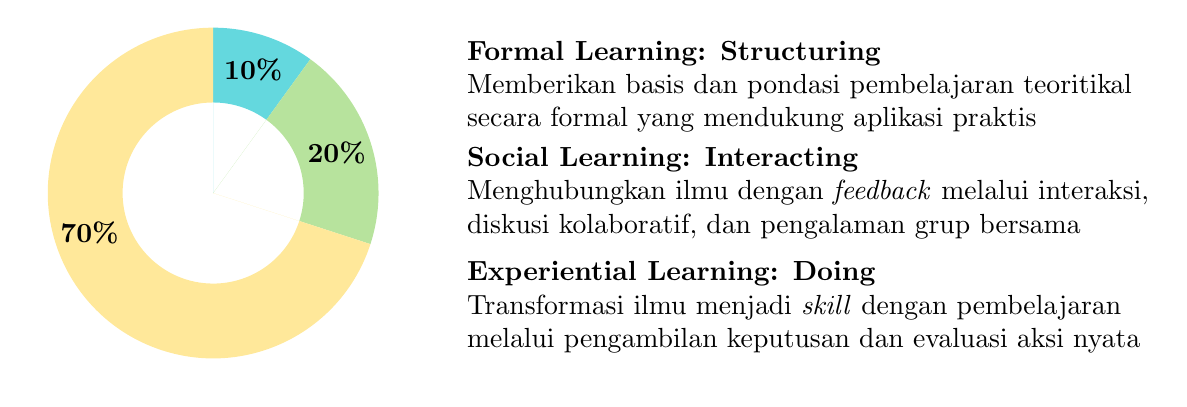
\begin{tikzpicture}
\def\R{2.1}\def\r{1.15}
\path[fill=cyanlearn] (0,0) -- (90:\R) arc (90:54:\R) -- (54:\r) arc (54:90:\r) -- cycle;
\path[fill=greenlearn] (0,0) -- (54:\R) arc (54:-18:\R) -- (-18:\r) arc (-18:54:\r) -- cycle;
\path[fill=yellowlearn] (0,0) -- (-18:\R) arc (-18:-270:\R) -- (-270:\r) arc (-270:-18:\r) -- cycle;
\node[font=\bfseries] at (72:1.65) {10\%};
\node[font=\bfseries] at (18:1.65) {20\%};
\node[font=\bfseries] at (198:1.65) {70\%};
\node[anchor=west,align=left] at (3.1,1.35) {\textbf{Formal Learning: Structuring}\\Memberikan basis dan pondasi pembelajaran teoritikal\\secara formal yang mendukung aplikasi praktis};
\node[anchor=west,align=left] at (3.1,0) {\textbf{Social Learning: Interacting}\\Menghubungkan ilmu dengan \emph{feedback} melalui interaksi,\\diskusi kolaboratif, dan pengalaman grup bersama};
\node[anchor=west,align=left] at (3.1,-1.45) {\textbf{Experiential Learning: Doing}\\Transformasi ilmu menjadi \emph{skill} dengan pembelajaran\\melalui pengambilan keputusan dan evaluasi aksi nyata};
\end{tikzpicture}
\end{center}

\visualexplanation{The ring allocates 10 percent to formal learning, 20 percent to social learning, and 70 percent to experiential learning. The accompanying text links each share to a distinct function: formal learning structures the theoretical foundation, social learning develops understanding through feedback and shared interaction, and experiential learning turns knowledge into skill through decisions and evaluation of real action. The largest yellow sector therefore represents the program's emphasis on learning by doing.}

\section{Learning Architecture and Methodology}

\subsection{Learning Architecture: dari Cohort ke Small Group}

\begin{center}
\resizebox{0.97\textwidth}{!}{%
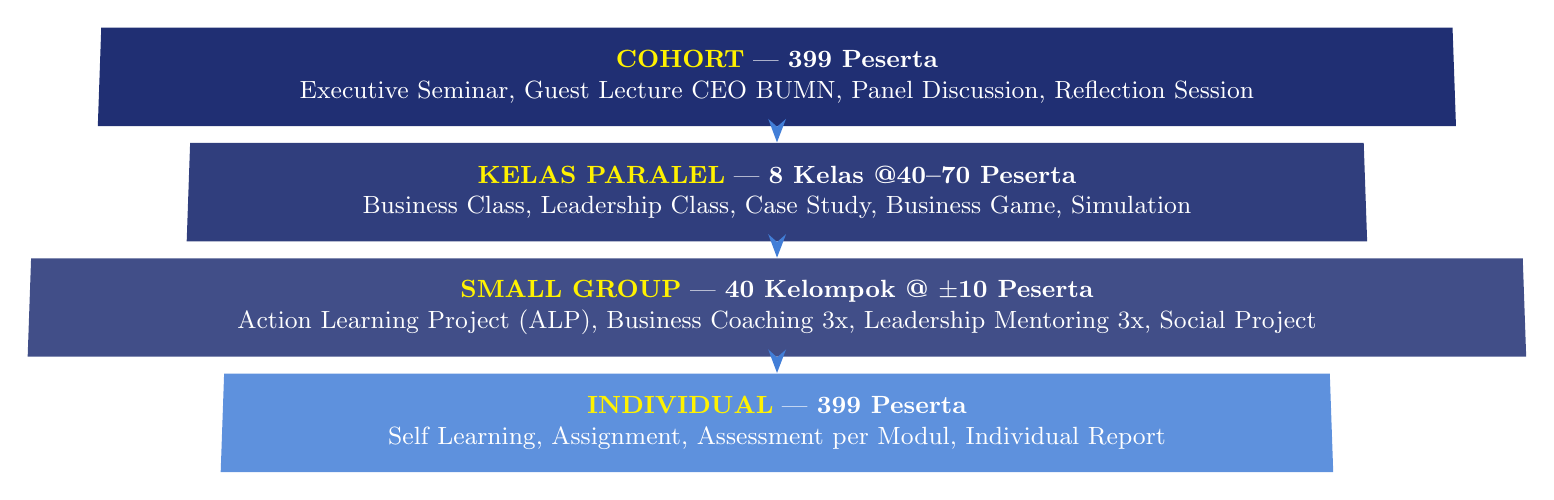
\begin{tikzpicture}[node distance=2mm, every node/.style={align=center,font=\small}]
\node[trapezium,trapezium left angle=88,trapezium right angle=88,fill=navy,text=white,minimum width=14.3cm,minimum height=1.25cm] (cohort) {\textbf{\color{yellow}COHORT} --- \textbf{399 Peserta}\\Executive Seminar, Guest Lecture CEO BUMN, Panel Discussion, Reflection Session};
\node[trapezium,trapezium left angle=88,trapezium right angle=88,fill=navy!93,text=white,minimum width=12.5cm,minimum height=1.25cm,below=of cohort] (class) {\textbf{\color{yellow}KELAS PARALEL} --- \textbf{8 Kelas @40--70 Peserta}\\Business Class, Leadership Class, Case Study, Business Game, Simulation};
\node[trapezium,trapezium left angle=88,trapezium right angle=88,fill=navy!85,text=white,minimum width=10.7cm,minimum height=1.25cm,below=of class] (group) {\textbf{\color{yellow}SMALL GROUP} --- \textbf{40 Kelompok @ $\pm$10 Peserta}\\Action Learning Project (ALP), Business Coaching 3x, Leadership Mentoring 3x, Social Project};
\node[trapezium,trapezium left angle=88,trapezium right angle=88,fill=midblue!85,text=white,minimum width=8.8cm,minimum height=1.25cm,below=of group] (individual) {\textbf{\color{yellow}INDIVIDUAL} --- \textbf{399 Peserta}\\Self Learning, Assignment, Assessment per Modul, Individual Report};
\draw[-{Stealth},very thick,midblue] (cohort)--(class);
\draw[-{Stealth},very thick,midblue] (class)--(group);
\draw[-{Stealth},very thick,midblue] (group)--(individual);
\end{tikzpicture}
}
\end{center}

\visualexplanation{The narrowing architecture moves from experiences shared by all 399 participants to increasingly focused learning contexts. The whole cohort attends executive seminars, guest lectures, panel discussions, and reflection. Eight parallel classes of 40--70 participants conduct business and leadership classes, cases, games, and simulations. Those classes divide into 40 groups of approximately ten for ALP work, coaching, mentoring, and the Social Project. At the narrowest level, every participant completes self-learning, assignments, module assessments, and an individual report.}

\subsection{Core Learning Methodology}

\begin{tcolorbox}[colback=lightgray,colframe=lightgray,arc=4mm]
\begin{tabularx}{\linewidth}{Y Y}
\textbf{\emph{Learning Methodology 1:}}\\
\textbf{6-Core Courses}\\
MK1 - Organizational Behavior \& Managing People,\\
MK2 - Financial Management \& Strategy,\\
MK3 - Marketing Management,\\
MK4 - Operations \& Supply Chain Management,\\
MK5 - Decision Making \& Negotiation,\\
MK6 - Business Analytics
&
\textbf{\emph{Learning Methodology 2:}}\\
\textbf{ALP + Business Immersion + Social Project}\\[2mm]
Tantangan pada bisnis nyata dengan dampak terukur
\end{tabularx}
\end{tcolorbox}

\visualexplanation{The methodology has two complementary halves. Six core courses provide disciplinary knowledge across people, finance, marketing, operations, decision making, negotiation, and analytics. ALP, Business Immersion, and the Social Project then place that knowledge inside measurable real-business challenges.}

\subsection{Why Action Learning Project (ALP)?}

\begin{tcolorbox}[colback=lightgray,colframe=lightgray,arc=4mm]
\centering
\textbf{\color{navy}Action Learning Project (ALP) --- ``Learning through real business challenges with measurable impact''}\\[2mm]
\begin{tabularx}{\linewidth}{>{\centering\arraybackslash}Y >{\centering\arraybackslash}Y >{\centering\arraybackslash}Y}
\Large\textbf{Equip \& Transform Participants Capability} &
\Large\textbf{Real Business ROI that Creates Value} &
\Large\textbf{True Test of Agility \& Resilience}
\end{tabularx}
\end{tcolorbox}

\begin{tabularx}{\textwidth}{Y Y}
\begin{tcolorbox}[colback=lightgray,colframe=lightgray,arc=4mm,title=The Carpenter Analogy,fonttitle=\Large\bfseries\color{navy}]
\emph{``Tukang bangunan yang tahu menggunakan alat, belum tentu bisa membuat rumah. Hanya pengalaman dalam membuat rumah maka ia dapat menggunakan keahliannya.''}
\begin{itemize}
\item Can this person manage ambiguity, not just structured tasks?
\item Can they work together under real-time pressure?
\item Are they ready for a bigger, less-defined mandate?
\end{itemize}
\end{tcolorbox}
&
\begin{tcolorbox}[colback=lightgray,colframe=lightgray,arc=4mm,title={An ALP is a ``stretch'' assignment},fonttitle=\Large\bfseries\color{navy}]
\begin{itemize}[label=\color{green}$\checkmark$]
\item A clear picture of the problem, grounded in data and interviews
\item A named set of options, with trade-offs made explicit
\item A prioritized, financially-aware recommendation
\item A view on what it takes to implement it
\item Producing analysis and \textbf{concrete, actionable recommendations} a sponsor can act on
\end{itemize}
\end{tcolorbox}
\end{tabularx}

\visualexplanation{The ALP graphic connects participant development with business value and a test of agility. The carpenter analogy argues that knowing tools is not the same as delivering a finished result; participants must use their knowledge under ambiguity, time pressure, and a less-defined mandate. The checklist specifies the expected evidence of that capability: a data-grounded problem definition, explicit options and trade-offs, a prioritized financially aware recommendation, an implementation view, and concrete recommendations that a sponsor can act on.}

\section{Learning Journey Timeline: 6-Core Courses}

\emph{6 Mata Kuliah dirancang untuk membekali pelajar dengan kemampuan Business Leadership, dilaksanakan di Kampus Nawasena}

\begin{tabularx}{\textwidth}{Y Y Y}
\begin{tcolorbox}[colback=blue!8,colframe=blue,title=MK1 - Organizational Behavior and Managing People,fonttitle=\bfseries]
\centering 14 Lecture @ 1 Sesi \quad $\vert$ \quad 14 Case @ 2 Sesi
\end{tcolorbox}&
\begin{tcolorbox}[colback=teal!8,colframe=teal,title=MK2 - Financial Management and Strategy,fonttitle=\bfseries]
\centering 14 Lecture @ 1 Sesi \quad $\vert$ \quad 14 Case @ 2 Sesi
\end{tcolorbox}&
\begin{tcolorbox}[colback=burgundy!8,colframe=burgundy,title=MK3 - Marketing Management,fonttitle=\bfseries]
\centering 14 Lecture @ 1 Sesi \quad $\vert$ \quad 13 Case @ 2 Sesi \quad $\vert$ \quad 1 Game @ 2 Sesi
\end{tcolorbox}\\
\begin{tcolorbox}[colback=brick!8,colframe=brick,title=MK4 - Operations and Supply Chain Management,fonttitle=\bfseries]
\centering 14 Lecture @ 1 Sesi \quad $\vert$ \quad 14 Case @ 2 Sesi \quad $\vert$ \quad 1 Game @ 2 Sesi
\end{tcolorbox}&
\begin{tcolorbox}[colback=orange!8,colframe=orange,title=MK5 - Decision Making and Negotiation,fonttitle=\bfseries]
\centering 14 Lecture @ 1 Sesi \quad $\vert$ \quad 7 Case @ 2 Sesi \quad $\vert$ \quad 7 Roleplay @ 2 Sesi
\end{tcolorbox}&
\begin{tcolorbox}[colback=gold!8,colframe=gold,title=MK6 - Business Analytics,fonttitle=\bfseries]
\centering 14 Lecture @ 1 Sesi \quad $\vert$ \quad 14 Case @ 2 Sesi
\end{tcolorbox}
\end{tabularx}

\visualexplanation{The six colored course cards compare the instructional mix. Every course has 14 lectures. MK1, MK2, MK4, and MK6 each have 14 cases; MK3 has 13 cases plus one game; MK4 also has one game; and MK5 combines seven cases with seven roleplays. Cases, games, and roleplays are shown as two-session activities, while each lecture is one session.}

\begin{center}
\scriptsize
\resizebox{\textwidth}{!}{%
\begin{tabular}{L{3.2cm}*{14}{c}}
\textbf{Alur Mingguan per MK} & \textbf{M1}&\textbf{M2}&\textbf{M3}&\textbf{M4}&\textbf{M5}&\textbf{M6}&\textbf{M7}&\textbf{M8}&\textbf{M9}&\textbf{M10}&\textbf{M11}&\textbf{M12}&\textbf{M13}&\textbf{M14}\\
\textbf{Perkuliahan} & \multicolumn{7}{c}{\cellcolor{midblue}\color{white}Blok 1 --- lecture tentang topik pembelajaran @ 1 sesi} & \multicolumn{7}{c}{\cellcolor{midblue}\color{white}Blok 2 --- lecture tentang topik pembelajaran @ 1 sesi}\\
\textbf{Case Study} & \multicolumn{7}{c}{\cellcolor{blue}\color{white}Intensif diskusi kasus @ 2 sesi} & \multicolumn{7}{c}{\cellcolor{blue}\color{white}Intensif diskusi kasus @ 2 sesi}\\
\textbf{Gamification} & \multicolumn{6}{c}{\cellcolor{lightgray}} & \cellcolor{red!75}\color{white}OSCM 2 Sesi & \multicolumn{6}{c}{\cellcolor{lightgray}} & \cellcolor{red!75}\color{white}Mkt 2 Sesi\\
\textbf{Ujian} & \multicolumn{7}{c}{\cellcolor{lightgray}} & \cellcolor{orange!80}\color{white}Mid Term & \multicolumn{5}{c}{\cellcolor{lightgray}} & \cellcolor{orange!80}\color{white}Final Term\\
\textbf{Guest Lecture CEO BUMN} & \multicolumn{2}{c}{\cellcolor{lightgray}} & \cellcolor{medgray}\color{white}1 & \multicolumn{4}{c}{\cellcolor{lightgray}} & \cellcolor{medgray}\color{white}2 & \multicolumn{5}{c}{\cellcolor{lightgray}} & \cellcolor{medgray}\color{white}3\\
\rowcolor{paleblue}\textbf{Titik Sinkronisasi} & \multicolumn{3}{c}{\textbullet\ Kick Off ALP} & \multicolumn{4}{c}{\textbullet\ Milestone 1} & \multicolumn{5}{c}{\textbullet\ Milestone 2} & \multicolumn{2}{c}{\textbullet\ Final Presentation}\\
\end{tabular}}
\end{center}

\visualexplanation{The weekly grid places two seven-week lecture-and-case blocks across M1--M14. OSCM gamification occurs in M7 and Marketing gamification in M14. The Mid Term sits at M8 and the Final Term at M14. Three CEO guest lectures occur in M3, M8, and M14. The synchronization band aligns the course sequence with the ALP: kick-off in the opening weeks, Milestone 1 near the end of the first block, Milestone 2 during the second block, and the final presentation at the end.}

\section{Learning Journey Timeline: Action Learning Project}

\emph{Enam tahap ALP SMART-gated di 10 BUMN mitra, dengan tiga milestone sebagai gerbang antar tahap ALP}

\begin{center}
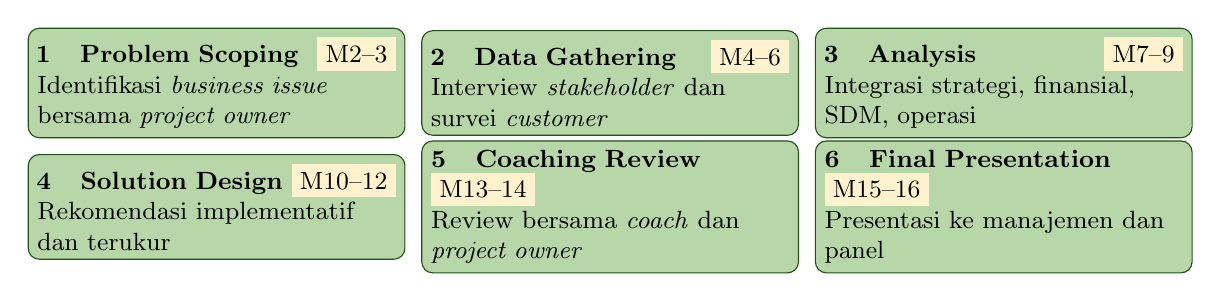
\begin{tikzpicture}[node distance=2mm and 2mm,every node/.style={font=\small}]
\node[draw=green!65!black,fill=palegreen,rounded corners,text width=4.55cm,minimum height=1.25cm] (s1) {\textbf{1\quad Problem Scoping}\hfill\colorbox{paleyellow}{M2--3}\\Identifikasi \emph{business issue} bersama \emph{project owner}};
\node[draw=green!65!black,fill=palegreen,rounded corners,text width=4.55cm,minimum height=1.25cm,right=of s1] (s2) {\textbf{2\quad Data Gathering}\hfill\colorbox{paleyellow}{M4--6}\\Interview \emph{stakeholder} dan survei \emph{customer}};
\node[draw=green!65!black,fill=palegreen,rounded corners,text width=4.55cm,minimum height=1.25cm,right=of s2] (s3) {\textbf{3\quad Analysis}\hfill\colorbox{paleyellow}{M7--9}\\Integrasi strategi, finansial, SDM, operasi};
\node[draw=green!65!black,fill=palegreen,rounded corners,text width=4.55cm,minimum height=1.25cm,below=of s1] (s4) {\textbf{4\quad Solution Design}\hfill\colorbox{paleyellow}{M10--12}\\Rekomendasi implementatif dan terukur};
\node[draw=green!65!black,fill=palegreen,rounded corners,text width=4.55cm,minimum height=1.25cm,right=of s4] (s5) {\textbf{5\quad Coaching Review}\hfill\colorbox{paleyellow}{M13--14}\\Review bersama \emph{coach} dan \emph{project owner}};
\node[draw=green!65!black,fill=palegreen,rounded corners,text width=4.55cm,minimum height=1.25cm,right=of s5] (s6) {\textbf{6\quad Final Presentation}\hfill\colorbox{paleyellow}{M15--16}\\Presentasi ke manajemen dan panel};
\end{tikzpicture}
\end{center}

\visualexplanation{The six-stage flow begins after the first month. Problem Scoping occupies M2--M3; Data Gathering, M4--M6; Analysis, M7--M9; Solution Design, M10--M12; Coaching Review, M13--M14; and Final Presentation, M15--M16. Each stage feeds the next, moving from issue definition and evidence to integrated analysis, an implementable recommendation, review, and presentation to management and the panel.}

\begin{center}
\scriptsize
\resizebox{\textwidth}{!}{%
\begin{tabular}{L{3.4cm}*{16}{c}}
\textbf{Alur Mingguan} & \textbf{M1}&\textbf{M2}&\textbf{M3}&\textbf{M4}&\textbf{M5}&\textbf{M6}&\textbf{M7}&\textbf{M8}&\textbf{M9}&\textbf{M10}&\textbf{M11}&\textbf{M12}&\textbf{M13}&\textbf{M14}&\textbf{M15}&\textbf{M16}\\
\textbf{Tahap ALP} & \cellcolor{lightgray} & \cellcolor{palegreen}Scoping & \cellcolor{palegreen}Scoping & \cellcolor{palegreen}Data Gathering & \cellcolor{palegreen}Data Gathering & \cellcolor{palegreen}Data Gathering & \cellcolor{palegreen}Analysis & \cellcolor{palegreen}Analysis & \cellcolor{palegreen}Analysis & \cellcolor{palegreen}Solution Design & \cellcolor{palegreen}Solution Design & \cellcolor{palegreen}Solution Design & \cellcolor{palegreen}Coaching Review & \cellcolor{palegreen}Coaching Review & \cellcolor{palegreen}Final Presentation & \cellcolor{palegreen}Final Presentation\\
\textbf{Mentoring Praktisi BUMN} & \cellcolor{lightgray} & \cellcolor{lightgray} & \cellcolor{blue}\color{white}1 & \cellcolor{lightgray} & \cellcolor{lightgray} & \cellcolor{lightgray} & \cellcolor{blue}\color{white}2 & \cellcolor{lightgray} & \cellcolor{lightgray} & \cellcolor{lightgray} & \cellcolor{blue}\color{white}3 & \cellcolor{lightgray} & \cellcolor{lightgray} & \cellcolor{lightgray} & \cellcolor{lightgray} & \cellcolor{lightgray}\\
\textbf{Coaching Akademisi} & \cellcolor{lightgray} & \cellcolor{lightgray} & \cellcolor{lightgray} & \cellcolor{blue}\color{white}1 & \cellcolor{lightgray} & \cellcolor{lightgray} & \cellcolor{lightgray} & \cellcolor{blue}\color{white}2 & \cellcolor{lightgray} & \cellcolor{lightgray} & \cellcolor{lightgray} & \cellcolor{blue}\color{white}3 & \cellcolor{lightgray} & \cellcolor{lightgray} & \cellcolor{lightgray} & \cellcolor{lightgray}\\
\textbf{Milestone} & \cellcolor{lightgray} & \cellcolor{lightgray} & \cellcolor{lightgray} & \cellcolor{lightgray} & \cellcolor{lightgray} & \cellcolor{orange!80}\color{white}M1 & \cellcolor{lightgray} & \cellcolor{lightgray} & \cellcolor{lightgray} & \cellcolor{lightgray} & \cellcolor{lightgray} & \cellcolor{orange!80}\color{white}M2 & \cellcolor{lightgray} & \cellcolor{lightgray} & \cellcolor{lightgray} & \cellcolor{orange!80}\color{white}M3\\
\textbf{Immersion \& Social Project} & \cellcolor{lightgray} & \cellcolor{lightgray} & \cellcolor{lightgray} & \cellcolor{lightgray} & \cellcolor{medgray}\color{white}Imm 1 & \cellcolor{lightgray} & \cellcolor{lightgray} & \cellcolor{lightgray} & \cellcolor{lightgray} & \cellcolor{lightgray} & \cellcolor{medgray}\color{white}Imm 2 & \cellcolor{lightgray} & \cellcolor{medgray}\color{white}Social & \cellcolor{medgray}\color{white}Project & \cellcolor{medgray}\color{white}Project & \cellcolor{lightgray}\\
\rowcolor{paleblue}\textbf{Titik Sinkronisasi} & & \shortstack{\textbullet\\Kick Off ALP} & & & & \shortstack{\textbullet\\Milestone 1} & & \shortstack{\textbullet\\Mid Term} & & & & \shortstack{\textbullet\\Milestone 2} & & & & \shortstack{\textbullet\\Final Presentation}\\
\end{tabular}}
\end{center}

\visualexplanation{The 16-week grid overlays support events and gates on the six ALP stages. Practitioner mentoring sessions are placed in M3, M7, and M11; academic coaching sessions in M4, M8, and M12; and formal milestones in M6, M12, and M16. Immersion activities occur in M5 and M11, followed by the Social Project in M13--M15. The synchronization row highlights the shared program checkpoints: ALP kick-off, Milestone 1, Mid Term, Milestone 2, and the Final Presentation.}

\section{Course Curriculum: MK1 -- Organizational Behaviour \& Managing People}

\subsection{Learning Outcomes}
\begin{itemize}
\item Understand how to collaborate with other parties
\item Concept of conflict management to solve problems in a small group learning environment
\item Demonstrate constructive feedback in a small group learning environment
\item Demonstrate the tendency to take the initiative
\item Students are able to influence others in their team
\item Inspire and empower others by evaluating, analyzing and providing criticism about how leadership behavior and characteristics affect workers and achievements in business
\item Demonstrate the ability to manage change
\end{itemize}

\begin{tabularx}{\textwidth}{Y Y}
\begin{tcolorbox}[colback=white,colframe=navy,title=Tim Pengajar - Dosen Pengampu,fonttitle=\bfseries]
Muhammad Yorga Permana, Ph.D.\\
Widhyawan Prawiraatmadja, Ph.D.\\
Dr. Ir. Madju Yuni Ros Bangun\\
Yudo Anggoro, Ph.D.
\end{tcolorbox}&
\begin{tcolorbox}[colback=white,colframe=midblue,title=Asisten Mata Kuliah,fonttitle=\bfseries]
Efryta Wulan (081245103149)
\end{tcolorbox}
\end{tabularx}

\begin{center}\small
\begin{tabularx}{\textwidth}{c L{5.0cm} Y}
\rowcolor{navy}\color{white}\bfseries Minggu & \color{white}\bfseries Topik & \color{white}\bfseries Sub-Topik\\
1 & Understanding Self \& Leading Others & Strategizing Your Life: Self-Awareness, Values \& Purpose\\
2 & Understanding Self \& Leading Others & Who Am I at Work? Identity, Personality \& Individual Differences\\
3 & Understanding Self \& Leading Others & Motivation \& Human Behavior at Work\\
4 & Understanding Self \& Leading Others & Leadership \& Influence\\
5 & Navigating Teams \& Organizations & Team Dynamics, Communication, Negotiation \& Conflict\\
6 & Navigating Teams \& Organizations & Organizational Culture\\
7 & Navigating Teams \& Organizations & Power \& Politics in Organizations\\
8 & Building the Organization \& Talent & People \& Strategy: Human Capital as Competitive Advantage\\
9 & Building the Organization \& Talent & Organization Design \& Strategic Workforce Planning\\
10 & Building the Organization \& Talent & Strategic Talent Acquisition \& Employer Branding\\
11 & Building the Organization \& Talent & Talent Management, Development \& Succession\\
12 & Driving Performance \& Transformation & Performance Management, Compensation, and Benefits\\
13 & Driving Performance \& Transformation & Leading Change, Transformation \& the Future of the Workplace\\
14 & Driving Performance \& Transformation & Employee Experience, Engagement \& Inclusion\\
\end{tabularx}
\end{center}

\visualexplanation{The curriculum progresses through four topic blocks. Weeks 1--4 develop self-understanding and leadership; Weeks 5--7 move into team dynamics, culture, power, and politics; Weeks 8--11 address organization design and talent systems; and Weeks 12--14 connect performance management with change, the future of the workplace, and employee experience. This sequence supports the stated outcomes by moving from individual behavior to team influence and then to organization-wide transformation.}

\section{Course Curriculum: MK2 -- Financial Management and Strategy}

\subsection{Learning Outcomes}
\begin{itemize}
\item Demonstrate understanding of the financial management function and the firm's financial goals.
\item Conduct analytical reviews of financial statements and projections; apply time-value-of-money concepts and techniques.
\item Apply tools to analyze financial decisions---investment, financing, payout, and working capital---and address real-world financial issues.
\item Identify the financial environment and institutions; recognize the importance of ethics in financial decision making.
\end{itemize}

\begin{tabularx}{\textwidth}{Y Y}
\begin{tcolorbox}[colback=white,colframe=navy,title=Tim Pengajar - Dosen Pengampu,fonttitle=\bfseries]
Dr. Arif Zamani\\Dr. Subiakto Soekarno\\Dr. Aswin Rahadi\\Yunieta Anny Nainggolan, Ph.D.\\Oktofa Yudha Sudrajat, Ph.D.
\end{tcolorbox}&
\begin{tcolorbox}[colback=white,colframe=midblue,title=Asisten Mata Kuliah,fonttitle=\bfseries]
Annisa Rizkia Syaputri (081809905646)
\end{tcolorbox}
\end{tabularx}

\begin{center}\small
\begin{tabularx}{\textwidth}{c L{5.0cm} Y}
\rowcolor{navy}\color{white}\bfseries Minggu & \color{white}\bfseries Topik & \color{white}\bfseries Sub-Topik\\
1 & Financial Foundations & Financial Management Function \& Objectives\\
2 & Financial Foundations & Financial Statement Analysis\\
3 & Financial Foundations & Financial Statement Projections\\
4 & Cost \& Managerial Accounting & Management Accounting Fundamentals\\
5 & Cost \& Managerial Accounting & Cost Analysis \& Activity-Based Costing\\
6 & Time Value of Money & Time Value of Money (1)\\
7 & Time Value of Money & Time Value of Money (2)\\
8 & Corporate Financial Decisions & Capital Budgeting (1)\\
9 & Corporate Financial Decisions & Capital Budgeting (2)\\
10 & Corporate Financial Decisions & Pay-Out Policy\\
11 & Corporate Financial Decisions & Financing Decisions \& Financial Environment\\
12 & Corporate Financial Decisions & Working Capital Management\\
13 & Financial Risk Management & Definition of risk, risk-return relationship, \& risk governance\\
14 & Ethics \& Synthesis & Group Project Presentations\\
\end{tabularx}
\end{center}

\visualexplanation{The table begins with the financial statements and management objectives needed for analysis, then adds managerial accounting and time-value-of-money tools. Weeks 8--12 form the central corporate-decision block, covering capital budgeting, payout, financing, and working capital. Risk management in Week 13 and the ethics-and-synthesis presentation in Week 14 connect the analytical tools to responsible financial judgment.}

\section{Course Curriculum: MK3 -- Marketing Management}

\subsection{Learning Outcomes}
\begin{itemize}
\item Identifying and analyzing the core marketing problems in a business case.
\item Identifying ethical marketing issues in a business case.
\item Taking initiative in the process of designing a Marketing Plan.
\item In groups, students are able to identify and analyze the core marketing problems in the process of evaluating a Marketing Plan design.
\end{itemize}

\begin{tabularx}{\textwidth}{Y Y}
\begin{tcolorbox}[colback=white,colframe=navy,title=Tim Pengajar - Dosen Pengampu,fonttitle=\bfseries]
Ira Fachira, Ph.D.\\Atik Aprianingsih, DBA\\Ilma Aulia Zaim, Ph.D.\\Nila Armelia, Ph.D.\\Dr. Gallang Perdhana Dalimunthe
\end{tcolorbox}&
\begin{tcolorbox}[colback=white,colframe=midblue,title=Asisten Mata Kuliah,fonttitle=\bfseries]
Nia Desiana (081214533663)
\end{tcolorbox}
\end{tabularx}

\begin{center}\small
\begin{tabularx}{\textwidth}{c L{5.0cm} Y}
\rowcolor{navy}\color{white}\bfseries Minggu & \color{white}\bfseries Topik & \color{white}\bfseries Sub-Topik\\
1 & Foundations & Creating Customer Value\\
2 & Foundations & Analyzing the Marketing Environment\\
3 & Customer \& Market Insight & Managing Marketing Information \& Customer Insights (1)\\
4 & Customer \& Market Insight & Managing Marketing Information \& Customer Insights (2)\\
5 & Customer \& Market Insight & Marketing Research\\
6 & STP Strategy & Segmentation \& Targeting\\
7 & STP Strategy & Positioning\\
8 & STP Strategy & Games: Selling\\
9 & Marketing Mix (4Ps) & Marketing Mix --- Product \& Services\\
10 & Marketing Mix (4Ps) & Marketing Mix --- Price\\
11 & Marketing Mix (4Ps) & Marketing Mix --- Place (Channel) \& Digital Marketing\\
12 & Marketing Mix (4Ps) & Marketing Mix --- Promotion\\
13 & Branding \& Synthesis & Branding\\
14 & Branding \& Synthesis & Special Topic / Guest Lecture\\
\end{tabularx}
\end{center}

\visualexplanation{The course advances from customer value and the marketing environment to information, insights, and research. Weeks 6--8 build segmentation, targeting, positioning, and selling practice. Weeks 9--12 cover the four-part marketing mix of product and services, price, place and digital channels, and promotion. Branding and a special topic or guest lecture complete the synthesis, giving the Marketing Plan outcomes a week-by-week analytical structure.}

\section{Course Curriculum: MK4 -- Operations and Supply Chain Management}

\subsection{Learning Outcomes}
\begin{itemize}
\item Students will be able to demonstrate an understanding of theory, concepts, models or reasoning in operations and supply chain management related to specific problems/issues/contexts as discussed throughout the course.
\item Students will be able to critique concepts, models or reasoning in operations and supply chain management, so as to suggest solutions and managerial recommendations.
\item Students will understand the role of operations and supply chain management within the global business context.
\end{itemize}

\begin{tabularx}{\textwidth}{Y Y}
\begin{tcolorbox}[colback=white,colframe=navy,title=Tim Pengajar - Dosen Pengampu,fonttitle=\bfseries]
Noorhan Firdaus Pambudi, Ph.D.\\Dr. Yuanita Handayati\\Berty Argiyantari, Ph.D.\\Dr. Liane Okdinawati
\end{tcolorbox}&
\begin{tcolorbox}[colback=white,colframe=midblue,title=Asisten Mata Kuliah,fonttitle=\bfseries]
Laisa Aritonang (081221712180)
\end{tcolorbox}
\end{tabularx}

\begin{center}\small
\begin{tabularx}{\textwidth}{c L{5.0cm} Y}
\rowcolor{navy}\color{white}\bfseries Minggu & \color{white}\bfseries Topik & \color{white}\bfseries Sub-Topik\\
1 & Strategy and Product Design & Introduction to Operations and Supply Chain Management\\
2 & Strategy and Product Design & Strategy\\
3 & Strategy and Product Design & Product and Service Design\\
4 & Strategy and Product Design & Projects\\
5 & Capacity and Process & Strategic Capacity Planning\\
6 & Capacity and Process & Process Design and Analysis\\
7 & Capacity and Process & Waiting Line Analysis and Simulation\\
8 & Quality Assurance & Lean Operations\\
9 & Quality Assurance & Lean Six Sigma\\
10 & Quality Assurance & Statistical Quality Control\\
11 & Demand Fulfillment & Forecasting\\
12 & Demand Fulfillment & Sales \& Operations Planning\\
13 & Demand Fulfillment & Inventory Management\\
14 & Demand Fulfillment & MRP and ERP\\
\end{tabularx}
\end{center}

\visualexplanation{The operations sequence moves through four connected systems. Strategy and product design establish what the operation must deliver; capacity and process topics determine how work will flow; quality assurance introduces lean operations, Lean Six Sigma, and statistical control; and demand fulfillment links forecasts to sales and operations planning, inventory, MRP, and ERP. The table therefore follows the operational chain from strategic design through coordinated delivery.}

\section{Course Curriculum: MK5 -- Problem Solving, Decision Making and Negotiation}

\subsection{Learning Outcomes}
\begin{itemize}
\item Identifying and analyzing the core problems in a business case.
\item Building multiple perspectives by integrating various factors, relevant business functions, \& contextual information.
\item Developing solution options based on the perspectives built and the intended vision.
\item Making decisions based on the solution options developed.
\item Collaborating effectively with others.
\item Applying conflict management concepts to resolve problems within a team.
\item Providing constructive feedback within a team.
\item Communicating persuasively to influence and convince others.
\end{itemize}

\begin{tabularx}{\textwidth}{Y Y}
\begin{tcolorbox}[colback=white,colframe=navy,title=Tim Pengajar - Dosen Pengampu,fonttitle=\bfseries]
Dr. Valid Hasyimi\\Prof. Dr. Ir. Utomo Sarjono Putro\\Prof. Dr.Eng. Pri Hermawan\\Santi Novani, Ph.D.
\end{tcolorbox}&
\begin{tcolorbox}[colback=white,colframe=midblue,title=Asisten Mata Kuliah,fonttitle=\bfseries]
Syifa El-Baehaqi (08999230348)
\end{tcolorbox}
\end{tabularx}

\begin{center}\small
\begin{tabularx}{\textwidth}{c L{5.0cm} Y}
\rowcolor{navy}\color{white}\bfseries Minggu & \color{white}\bfseries Topik & \color{white}\bfseries Sub-Topik\\
1 & Foundations & Introduction to Negotiation\\
2 & Foundations & Rational Framework of Decision Making\\
3 & Kepner-Tregoe & Kepner-Tregoe Part 1\\
4 & Kepner-Tregoe & Kepner-Tregoe Part 2\\
5 & Kepner-Tregoe & Decision Analysis: SMART\\
6 & Kepner-Tregoe & Decision Analysis: AHP and Decision Tree\\
7 & Scenario Planning and Systems Thinking & Scenario Planning and Systems Thinking (1)\\
8 & Scenario Planning and Systems Thinking & Scenario Planning and Systems Thinking (2)\\
9 & Distributive Negotiation & Negotiation Dilemma\\
10 & Distributive Negotiation & Negotiation Style\\
11 & Distributive Negotiation & Claiming value (``Slicing the Pie'') in negotiation\\
12 & Integrative Negotiation & From distributive to integrative negotiation\\
13 & Integrative Negotiation & Integrative Negotiation Strategy and Technique\\
14 & Integrative Negotiation & Multiparty Negotiation \& Wrap Up\\
\end{tabularx}
\end{center}

\visualexplanation{The table links decision analysis and negotiation in a deliberate progression. Foundations introduce negotiation and rational decision making. The Kepner-Tregoe block adds SMART, AHP, and decision-tree analysis, followed by two weeks of scenario planning and systems thinking. The final six weeks move from distributive negotiation and claiming value to integrative strategy, technique, and multiparty negotiation, directly supporting the outcomes on multiple perspectives, options, collaboration, feedback, and persuasion.}

\section{Course Curriculum: MK6 -- Applied Business Analytics}

\subsection{Learning Outcomes}
\begin{itemize}
\item Identifying and analyzing the core problems in a business case.
\item Building multiple perspectives by integrating various factors, related business functions, and relevant contextual information.
\item Developing solution options based on the perspectives built and the intended vision.
\item Making decisions based on the solution options developed.
\end{itemize}

\begin{tabularx}{\textwidth}{Y Y}
\begin{tcolorbox}[colback=white,colframe=navy,title=Tim Pengajar - Dosen Pengampu,fonttitle=\bfseries]
Dr. Eng. Manahan Siallagan\\Dr. Shimaditya Nuraeni\\M. Apriandito Arya Saputra, MBA\\Bagus Rullym MM
\end{tcolorbox}&
\begin{tcolorbox}[colback=white,colframe=midblue,title=Asisten Mata Kuliah,fonttitle=\bfseries]
Tyas Larassati (081809230368)
\end{tcolorbox}
\end{tabularx}

\begin{center}\small
\begin{tabularx}{\textwidth}{c L{5.0cm} Y}
\rowcolor{navy}\color{white}\bfseries Minggu & \color{white}\bfseries Topik & \color{white}\bfseries Sub-Topik\\
1 & Foundations & Introduction to Business Analytics\\
2 & Foundations & Data-Driven Decision Making\\
3 & Foundations & Predictive Analytics for Business\\
4 & Applied Analytics & Customer Analytics\\
5 & Applied Analytics & Marketing Analytics\\
6 & Applied Analytics & Financial Analytics\\
7 & Applied Analytics & Supply Chain Analytics\\
8 & Applied Analytics & Risk Analytics\\
9 & Data \& Responsibility & Big Data in Business\\
10 & Data \& Responsibility & Ethical Considerations in Business Analytics\\
11 & Data \& Responsibility & Practical: Big Data Technologies\\
12 & Data \& Responsibility & Practical: Data Privacy and Security\\
13 & Advanced Analytics & Business Intelligence \& Visualization\\
14 & Advanced Analytics & Future Trends in Business Analytics\\
\end{tabularx}
\end{center}

\visualexplanation{The analytics curriculum starts with data-driven and predictive foundations, then applies analytics to customers, marketing, finance, supply chains, and risk. Weeks 9--12 place those applications inside a responsibility framework that covers big data, ethics, technology, privacy, and security. Business intelligence, visualization, and future trends form the advanced closing block, connecting analytical methods to business decisions and solution design.}

\end{document}
